\chapter{Modeling an Image Collection - Results}
\label{sec:results}

This chapter presents the results for different experiments performed on the datasets introduced in the previous chapter. Different models are evaluated and their outcome is discussed.

\section{The Problem with Singletons}

The histograms in Figures \ref{fig:histogram_path_length_10} and \ref{fig:histogram_path_length_100} show that most of the path datasets are composed on singleton paths representing users that only took photos around a small area on a single day. However, the evaluation procedure described in Section \ref{sec:evaluation} only deals with paths of at least 2 items, this represents a problem because the kind of data used for learning is not the same as for the evaluation phase. Moreover, initial experiments showed that the distribution of singleton paths is significantly different from that of paths with 2 or more elements.

In order to illustrate this, a special dataset only containing paths of length 2 or more was constructed. The log-modular model was then trained and evaluated on both versions of the datasets. This was done for both the small ($|V|=10$) and large ($|V|=100$) datasets.

The accuracy of the resulting models for the test data is shown in Figure \ref{fig:comparison_singletons_modular}. It shows that there is a significant improvement in the accuracy when only the distribution of non-singleton paths is considered for the log-modular model. This effect is also expected for the more complex models, e.g. FLID, because their initialization is based on the log-modular model. Note that for the Markov model there is no difference between including singletons or not because transition probabilities can only be learned from paths of 2 or more elements.

\begin{figure}
  \centering
  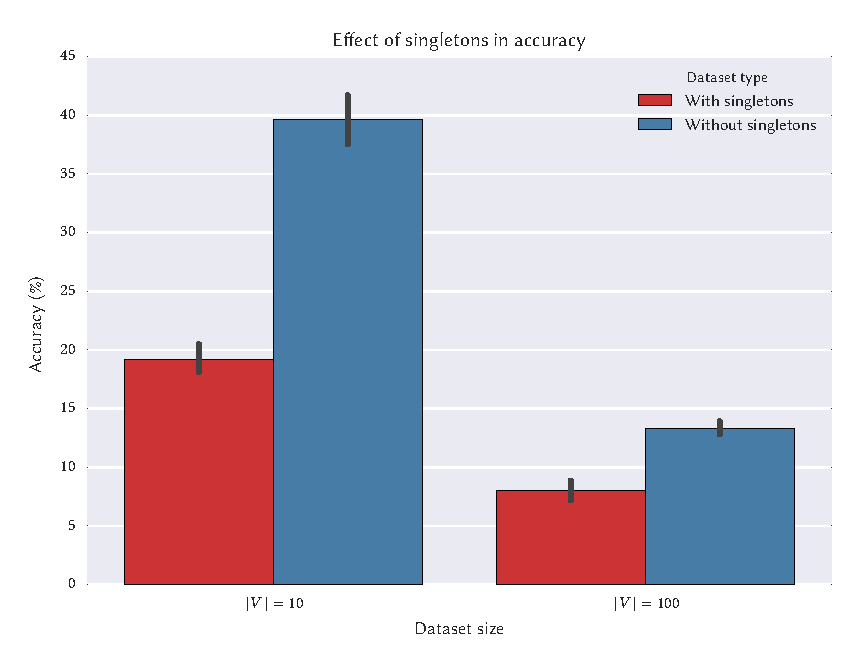
\includegraphics[width=\textwidth]{singletons_modular_comparison}
  \caption{Accuracy of log-modular models for different dataset configurations.}
  \label{fig:comparison_singletons_modular}
\end{figure}

Because of these results, the rest of the experiments were performed on the modified datasets without singletons which contain more significant data.

\section{Small Dataset}

First, the results from the baseline models are presented in Figure \ref{fig:small_baselines}. These show that the log-modular model outperforms the Markov baselines in this case. This is encouraging as it serves as the base for the more complex models. The results also show that the heuristic Markov model outperforms the strict Markov, this is expected in all cases because the dataset was constructed in such a way that elements are not repeated, hence the proposed heuristic always improves the prediction by removing the already visited elements from the possible choices. The proximity model is the best for the small dataset, and the different between the proximity model with and without ordering show that adding ordering information improves the score.

\begin{figure}
  \centering
  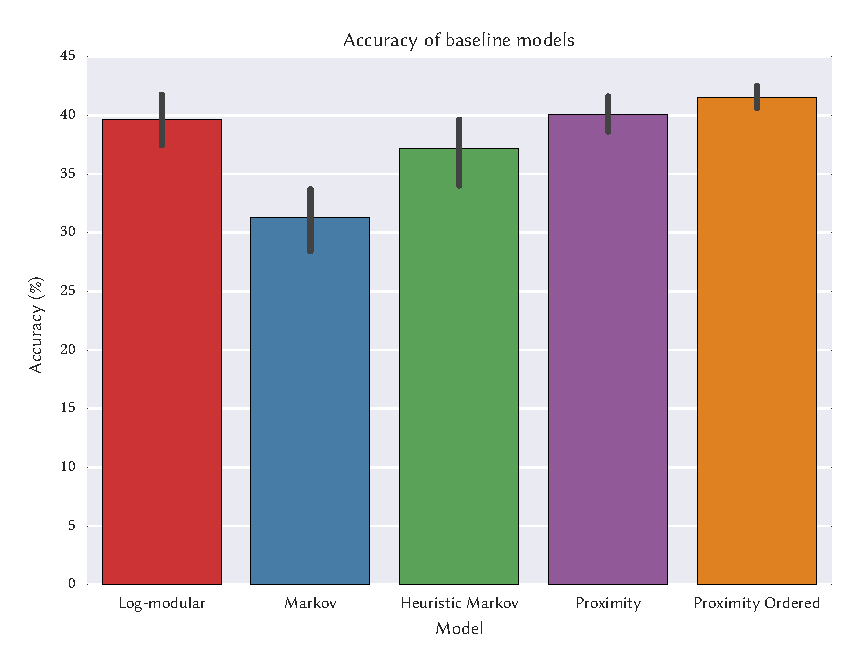
\includegraphics[width=\textwidth]{baseline_models_10}
  \caption{Accuracy of baseline models for the small dataset.}
  \label{fig:small_baselines}
\end{figure}

\subsection{Diversity \& Coherence}

The first approach to the problem was to use the FLID model, i.e. modeling only diversity. Figure \ref{fig:flid_small_l_dims} shows the model accuracy for different numbers of dimensions. Comparing these values with the log-modular model shows that there is no significant improvement even with a large number of diversity dimensions. Increasing the number of noise samples or epochs did not improve these results either.

\begin{figure}
  \centering
  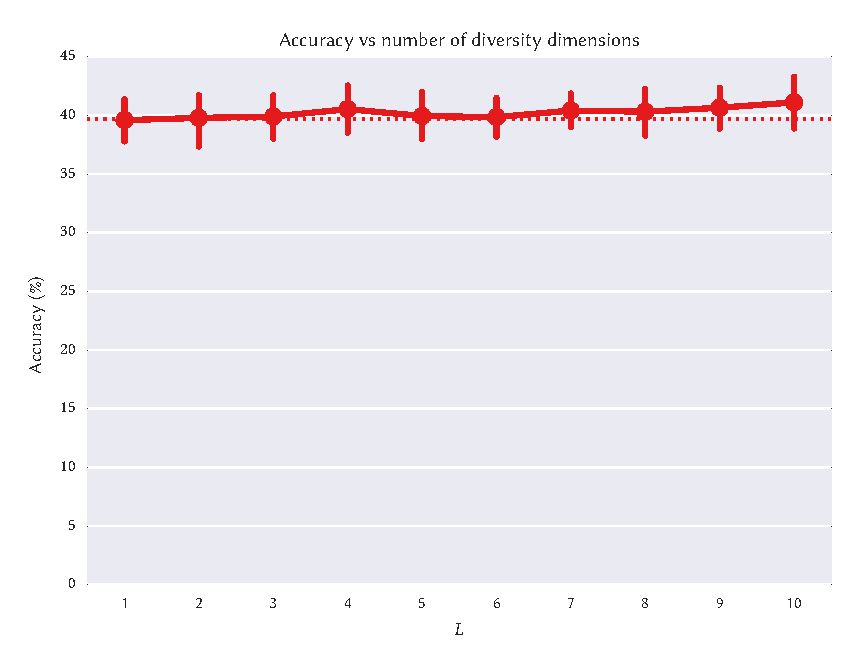
\includegraphics[width=\textwidth]{flid_10_l_dims}
  \caption{Accuracy for various values of $L$. The dotted line shows the mean accuracy of the log-modular model.}
  \label{fig:flid_small_l_dims}
\end{figure}

It is possible that for this dataset, diversity is not sufficient to capture the underlying distribution. Therefore, the next step was to use the FLDC model. After executing a grid search for $0 \geq L \geq 10$ and $0 \geq K \geq 0$ with the FLDC model the accuracy did not improve either.

The fact that the FLID and FLDC models do not result in improved accuracy with respect to the log-modular baseline can be explained by looking at the distribution of the paths in the data. The top 10 paths and their proportions in the dataset are listed in Table \ref{tab:small_top_paths}.

\begin{table}
  \centering
  \caption{Most frequent paths in the small Zürich dataset.}
  \begin{tabular}{@{}ll@{}}
    \toprule
    $S$ & $N(S)$\\
    \midrule
    $[1,4]$ & $71 (5.7\%)$ \\
    $[4,1]$ & $58 (4.7\%)$ \\
    $[6,1]$ & $47 (3.8\%)$ \\
    $[6,4]$ & $43 (3.5\%)$ \\
    $[1,6]$ & $37 (3.0\%)$ \\
    $[4,6]$ & $33 (2.6\%)$ \\
    $[2,4]$ & $26 (2.1\%)$ \\
    $[2,5]$ & $25 (2.0\%)$ \\
    $[5,2]$ & $24 (1.9\%)$ \\
    $[4,8]$ & $23 (1.8\%)$ \\
    \bottomrule
  \end{tabular}
  \label{tab:small_top_paths}
\end{table}

The paths in Table \ref{tab:small_top_paths} are all pairs, which are harder to predict because there is only information about one item. Simply ordering by frequency should give a high accuracy, as shown by the log-modular model's accuracy in Figure \ref{fig:small_baselines}.

However, the lack of improvement in accuracy does not mean that the FLID and FLDC models are not learning beyond the log-modular model. This can be seen by comparing the total variation distance between the empiric distribution of the paths, after removing the ordering, and the distributions produced by the learned models. Note that in this case the number of items is small enough that the computation of the partition function is tractable even using the exhaustive method that requires $\mathcal{O}(2^{|V|})$ time. Figure \ref{fig:small_tv_comparison} shows the total variation distance for different FLID and FLDC models. It shows that combining diversity and coherence improves the approximation of the model to the empiric distribution when compared to the TVD for the log-modular model, which was $0.40$.

Finally, Figure \ref{fig:small_llri} shows the LLRI metric for the FLDC models. This shows more clearly that there is an improvement over the log-modular model, even though it is not reflected on the accuracy metric. The best choice of dimensions is $L=5,K=5$ according to both the LLRI and TVD metrics.

\begin{figure}
  \centering
  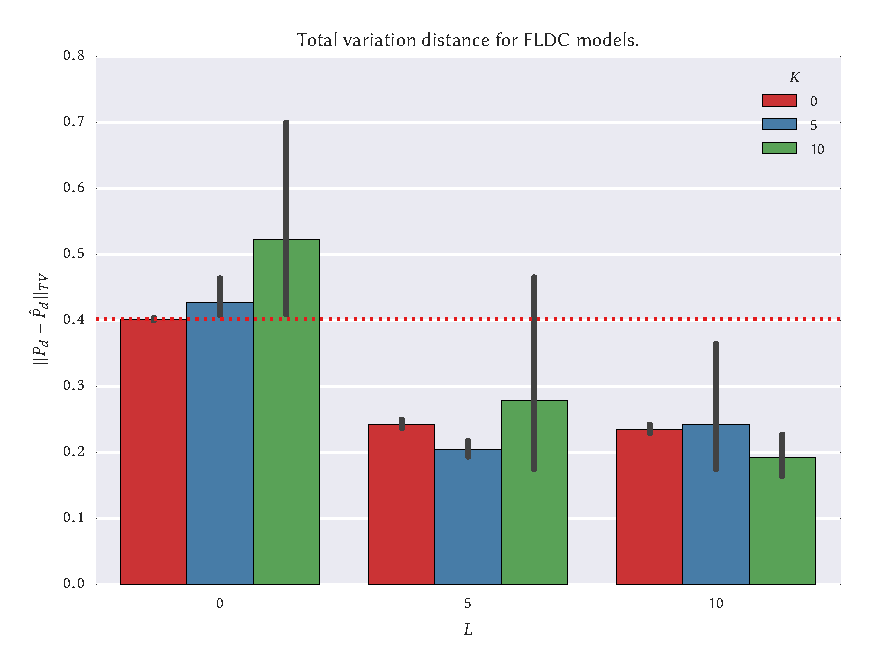
\includegraphics[width=\textwidth]{fldc_10_l_k_dims_tv}
  \caption{Total variation distance for FLDC models on the small dataset.}
  \label{fig:small_tv_comparison}
\end{figure}

\begin{figure}
  \centering
  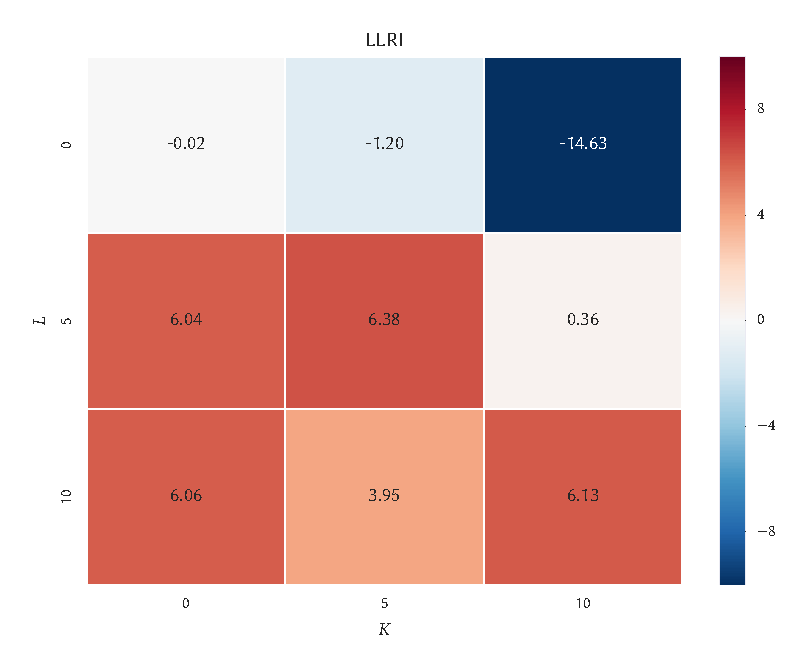
\includegraphics[width=\textwidth]{flid_10_llri}
  \caption{Log-likelihood relative improvement (LLRI) for FLDC models on the small dataset.}
  \label{fig:small_llri}
\end{figure}

\section{Large Dataset}

The baseline models were trained on the large dataset, i.e. $|V| = 100$, and the accuracy results are presented in Figure \ref{fig:all_models_100}. In this case, there is a more significant difference between the log-modular and the other baselines. This indicates that simply choosing the most frequent element is not as good of a strategy as for the small dataset, therefore complex models like FLDC and FFLDC should yield better results. Additionally, the significantly higher accuracy of the (Heuristic) Markov and Proximity Ordered models shows how adding information about the ordering, i.e. using paths, can improve the results in comparison to modeling only sets.

Different FLDC models were trained on the large dataset, in order to find the best setting for the dimensions $L$ and $K$ a grid search was performed. The average accuracy for each setting is presented in Figure \ref{fig:grid_search_large}. This shows that the FLDC model is significantly better for the path completion task than the log-modular baseline, however there is not a visible difference between the various settings for the model. Moreover, these results suggest that models with large number of dimensions have worse accuracy in the test set, this is due to the large number of parameters in the model which would require more data to estimate properly.

\begin{figure}
  \centering
  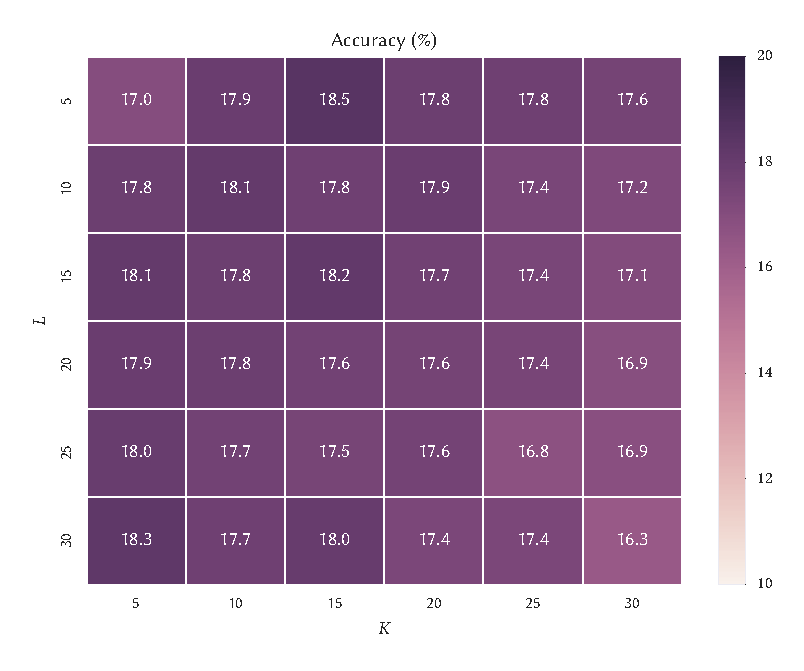
\includegraphics[width=\textwidth]{large_fldc_dims}
  \caption{Accuracy of FLDC models with varying $L$ and $K$ values.}
  \label{fig:grid_search_large}
\end{figure}

Finally, the best FLDC model is compared to the baselines in Figure \ref{fig:all_models_100}. Even though the FLDC model is an improvement over the log-modular, it still does not reach the accuracy of the Markov or Proximity Ordered models. This can be explained by the fact that the first three models in the figure include information about the order of the elements in a set, i.e. they model probabilities over paths, while the others only model membership of the elements in a set. This extra information helps these models perform the prediction task more accurately.

\begin{figure}
  \centering
  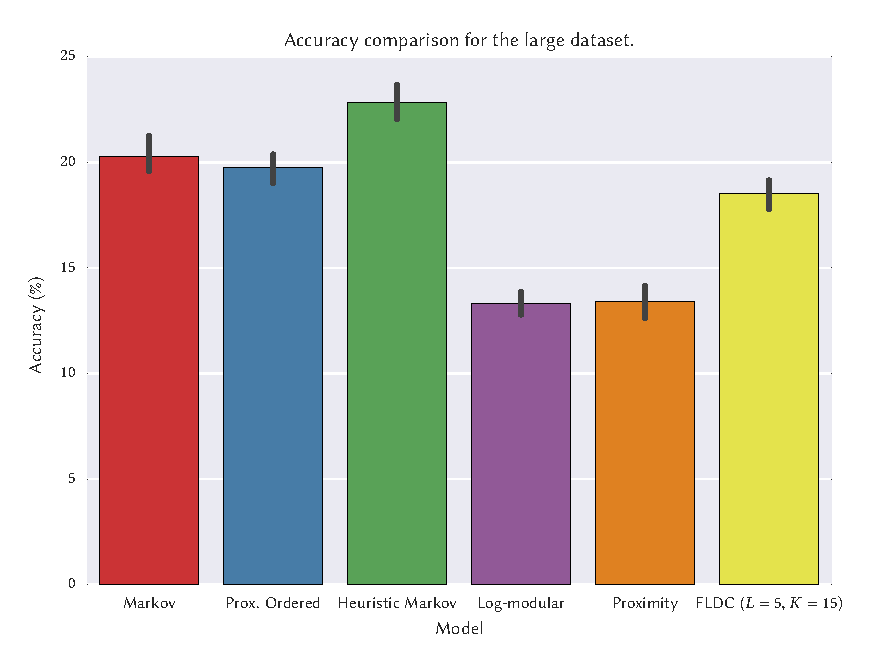
\includegraphics[width=\textwidth]{all_models_100}
  \caption{Comparison of baseline models to the best FLDC model for the large dataset.}
  \label{fig:all_models_100}
\end{figure}

Additional experiments with features were performed, aiming to enrich the model with information such as number of photos taken in a location and number of users. However, this did not show improvement in comparison to the FLDC model.